	\appendix

	\section{Layout}
		\subsection{Ring Oscillator}\label{sec:lay_osc}
			\subsubsection{Full oscillator layout}
				\begin{figure}[htb!]
				        \centering
				        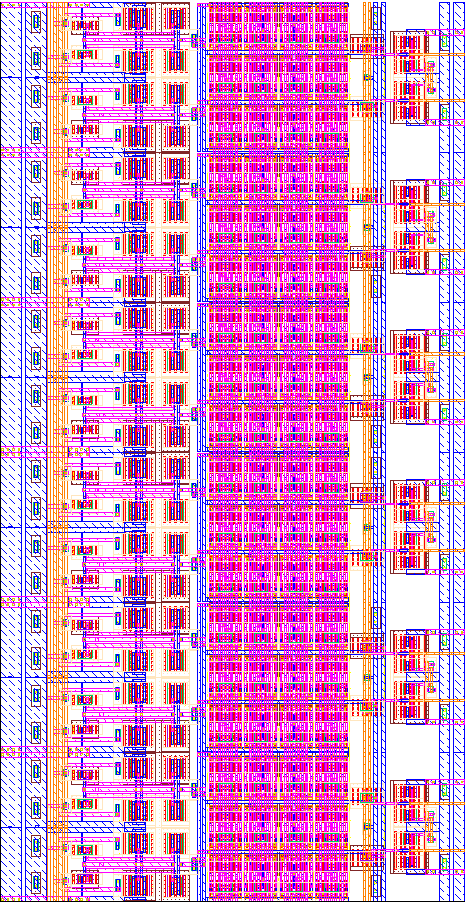
\includegraphics[height=0.75\textheight, angle=0]{./figs/layout/layout_osc}
				    \caption{Full six stage oscillator layout with capacitor tuning bank, reset switches, and output buffer.}
				\end{figure}
			\FloatBarrier\pagebreak
			\subsubsection{Pseudodifferential inverter delay cell}
				\begin{figure}[htb!]
				        \centering
				        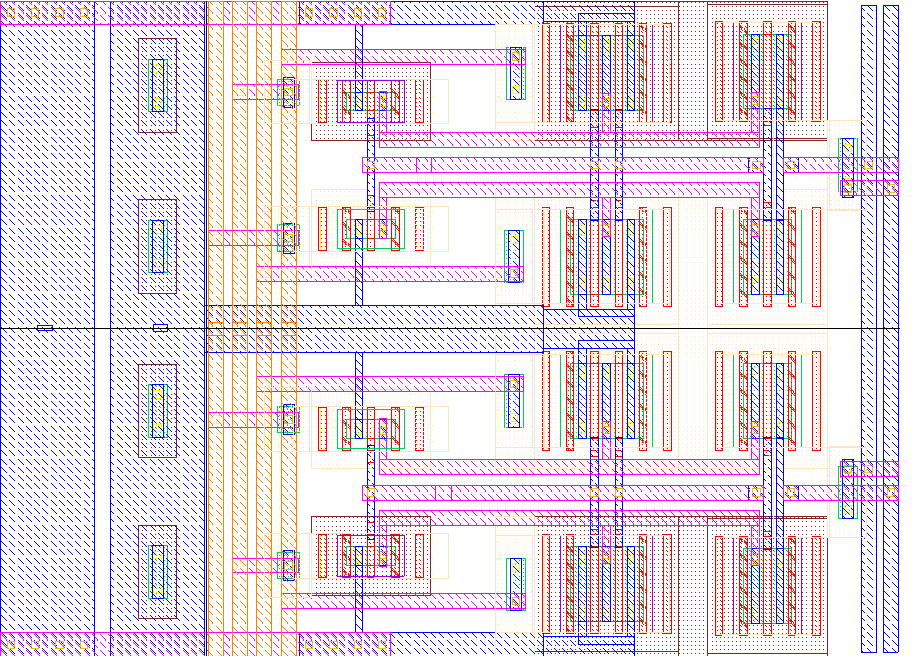
\includegraphics[width=0.8\textwidth, angle=0]{./figs/layout/layout_ro_pseudodiff_inv}
				    \caption{Unit delay stage pseudodifferential inverter.}
				\end{figure}
			\FloatBarrier
			\subsubsection{Capaitor tuning bank}
				\begin{figure}[htb!]
				        \centering
				        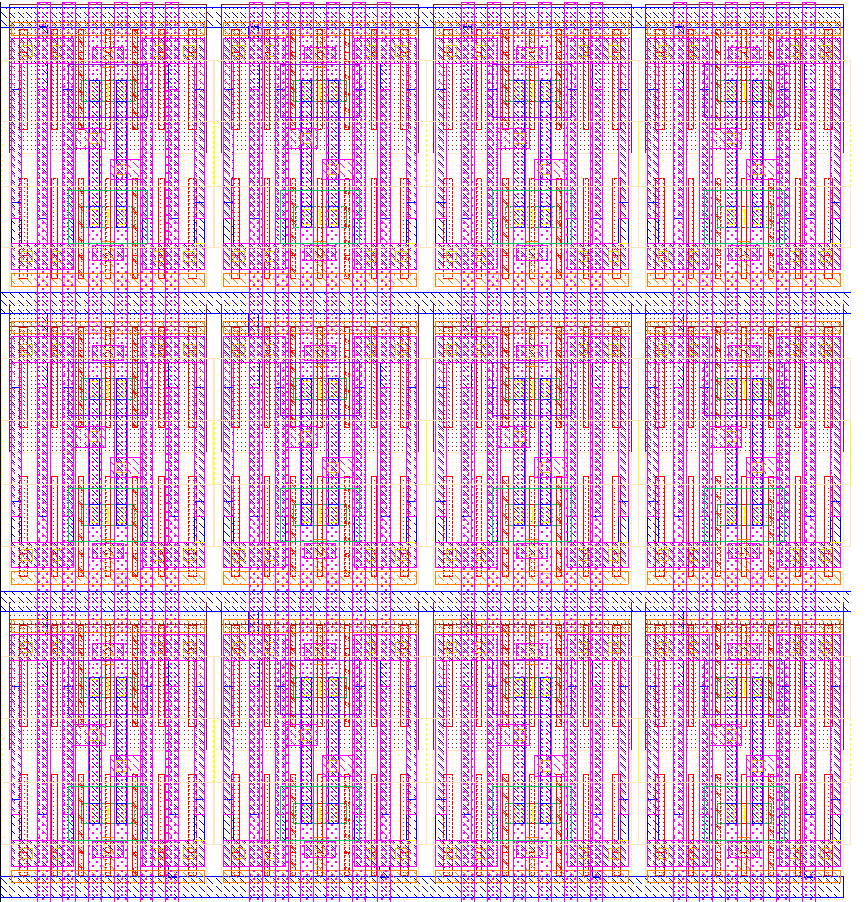
\includegraphics[width=0.6\textwidth, angle=0]{./figs/layout/layout_pvt_bank}
				    \caption{Capaitor tuning bank.}
				\end{figure}
		\FloatBarrier\pagebreak
		\subsection{10b CDAC}\label{sec:lay_cdac_10b}
			\subsubsection{Full CDAC Layout}
				\begin{figure}[htb!]
				        \centering
				        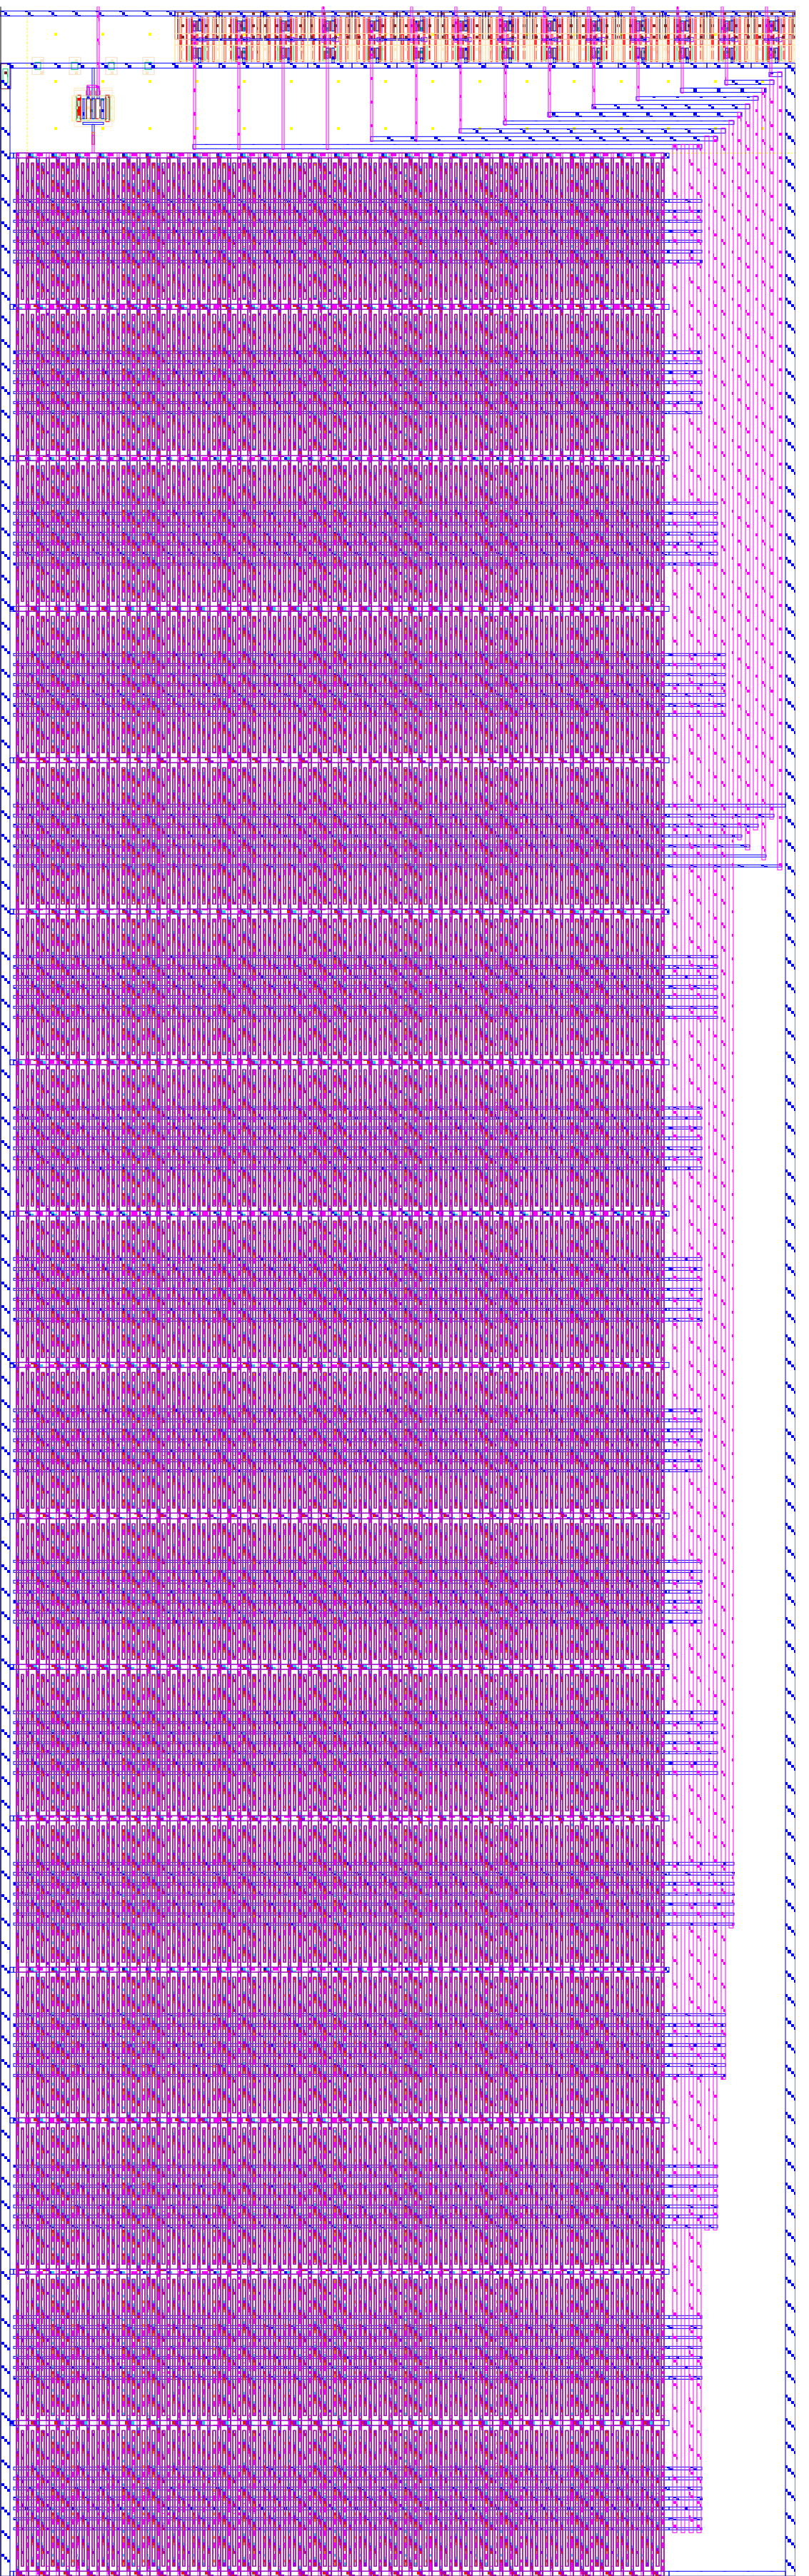
\includegraphics[height=0.85\textheight, angle=0]{./figs/layout/layout_cdac_10b}
				    \caption{10 bit CDAC layout.}
				\end{figure}
			\FloatBarrier\pagebreak
			\subsubsection{64 unit capacitor sub-bank}
				\begin{figure}[htb!]
				        \centering
				        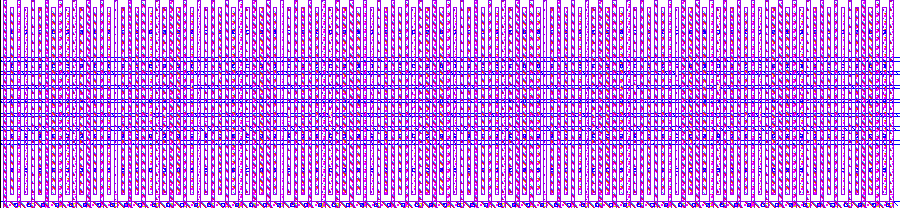
\includegraphics[width=\textwidth, angle=0]{./figs/layout/layout_cdac_unit_capbank}
				    \caption{64 unit capacitor bank.}
				\end{figure}
			\FloatBarrier
			\subsection{CDAC unit switch}
				\begin{figure}[htb!]
				        \centering
				        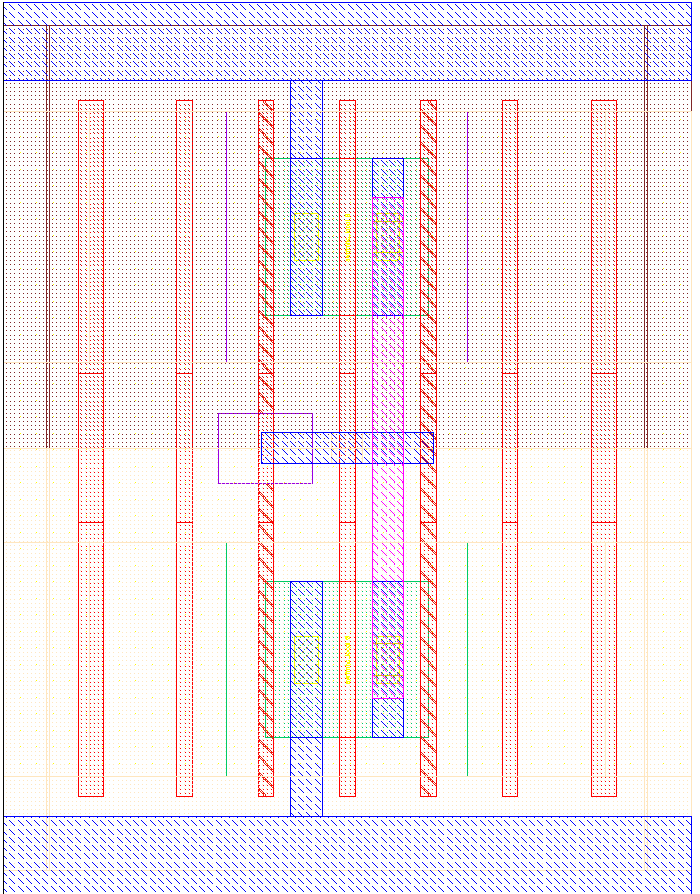
\includegraphics[width=0.5\textwidth, angle=0]{./figs/layout/layout_cdac_sw}
				    \caption{CDAC switch.}
				\end{figure}
		\FloatBarrier\pagebreak
		\subsection{3b CDAC}\label{sec:lay_cdac_3b}
			\begin{figure}[htb!]
			        \centering
			        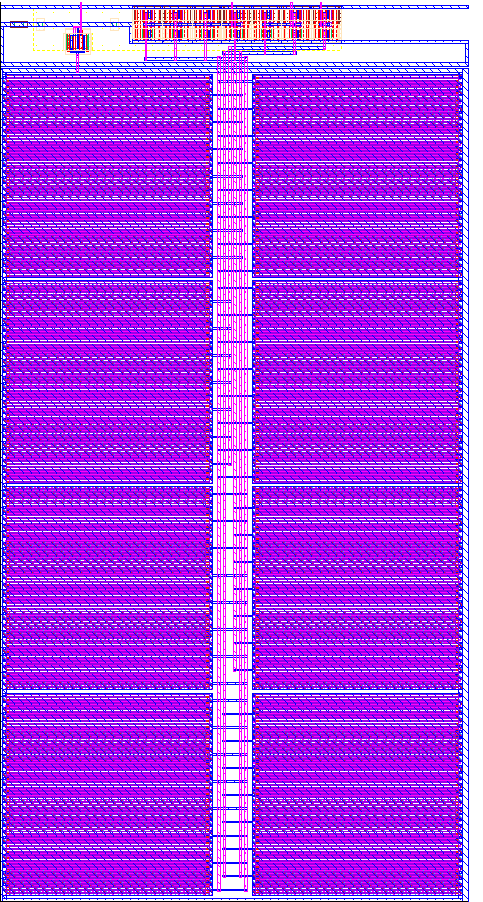
\includegraphics[height=0.85\textheight, angle=0]{./figs/layout/layout_cdac_3b}
			    \caption{3 bit CDAC layout.}
			\end{figure}
		\FloatBarrier\pagebreak
		\subsection{Buffer}\label{sec:lay_buff}
			\begin{figure}[htb!]
			        \centering
			        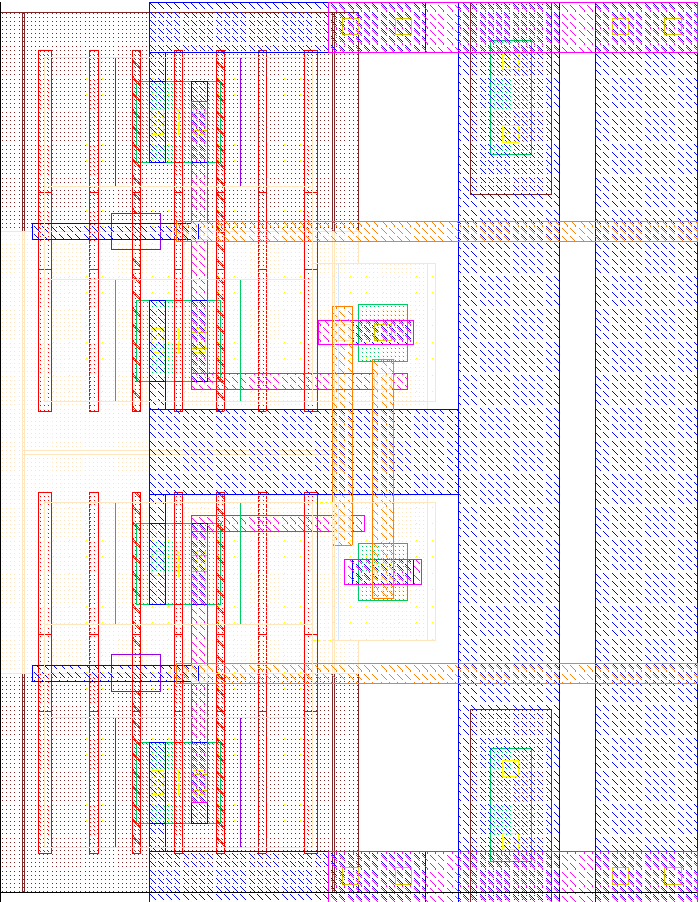
\includegraphics[width=0.8\textwidth, angle=0]{./figs/layout/layout_buffer}
			    \caption{Pseudodifferential inverter buffer cell.}
			\end{figure}
		\FloatBarrier\pagebreak
		\subsection{BBPD}\label{sec:lay_bbpd}
			\begin{figure}[htb!]
			        \centering
			        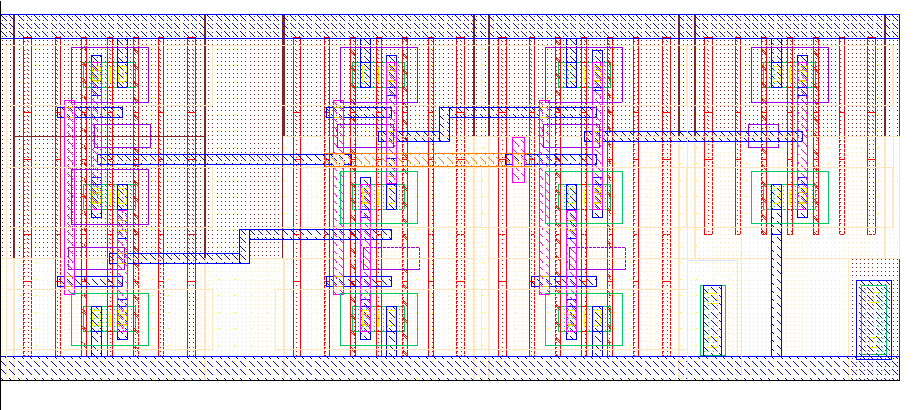
\includegraphics[width=\textwidth, angle=0]{./figs/layout/layout_bbpd}
			    \caption{Single ended bang-bang phase detector.}
			\end{figure}
			\begin{figure}[htb!]
			        \centering
			        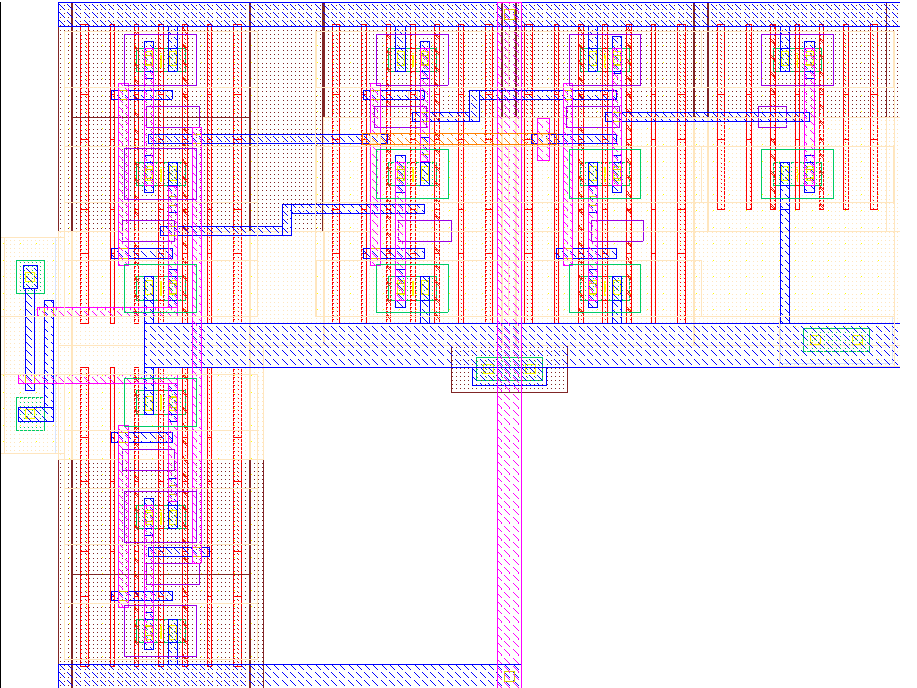
\includegraphics[width=\textwidth, angle=0]{./figs/layout/layout_bbpd_pseudodiff}
			    \caption{Pseudodifferential input bang-bang phase detector.}
			\end{figure}
		\FloatBarrier\pagebreak
		\subsection{SPNR Logic}
			\begin{figure}[htb!]
			        \centering
			        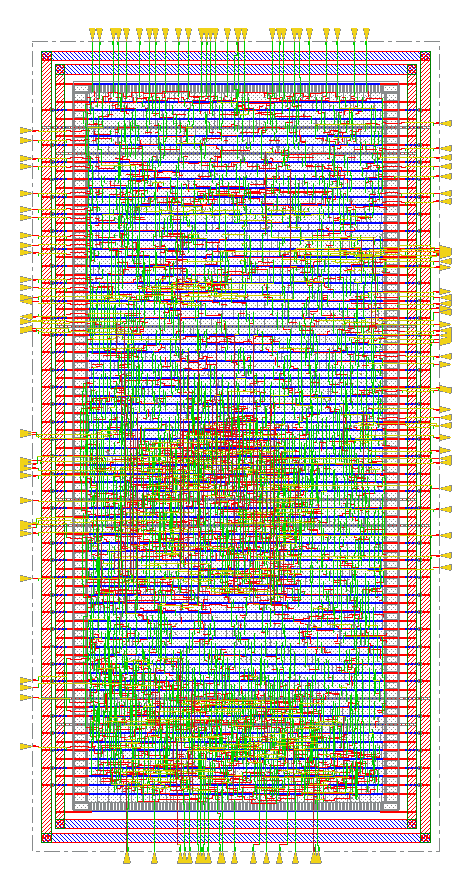
\includegraphics[height=0.8\textheight, angle=0]{./figs/layout/pnr_digital}
			    \caption{Place and route generated logic for PLL.}
			\end{figure}
		\FloatBarrier\pagebreak

	\section{Estimating PSD with Autoregressive Model}\label{yule_walker_ar_psd}
	The following is based on \cite{proakis_1993_psd}. Given a signal x[n] whose power spectrum should be estimated, its autocorrelation sequence $r_{xx}[l]$ with lag $l$ must be computed:
	\begin{equation}
		r_{xx}[l] = \sum_{n=-\infty}^{\infty} x[n]x[n-l]
	\end{equation}
	The autoregressive model for power spectrum, with p poles, that shall be fitted is given in \ref{eq:ar_psd_eq}
	\begin{equation}\label{eq:ar_psd_eq}
		S_{XX}(f) = \left.\frac{1}{|1+\sum_{n=1}^pa_nz^{-1}|^2}\right|_{z^{-1}=e^{-j2\pi f\Delta T}}
	\end{equation}
	MMSE optimization of the distribution for coefficients $\{a_1, ..., a_p\}$ is done by solving the Yule-Walker equation in \ref{eq:yule_walker}.
	\begin{equation} \label{eq:yule_walker}
	\begin{bmatrix}
	a_1\\ 
	a_2\\
	\vdots\\
	a_p
	\end{bmatrix} = 
	-\mathbf{R}_{xx}^{-1}\mathbf{r}_{xx}=
	-\begin{bmatrix}
	r_{xx}[0] & r_{xx}[1] & \dots & r_{xx}[p-1]\\ 
	r_{xx}[1] & r_{xx}[0] & \dots & r_{xx}[p-2]\\ 
	\vdots & \vdots &  & \\
	r_{xx}[p-1] & r_{xx}[p-2] &  & r_{xx}[0]
	\end{bmatrix}^{-1}
	\begin{bmatrix}
	r_{xx}[1]\\ 
	r_{xx}[2]\\
	\vdots\\
	r_{xx}[p]
	\end{bmatrix}
	\end{equation}

% \vspace{-0.8em}\center$ \square $
	% \section{Oscillator phase noise due to thermal noise}\label{osc_pn_additive_append}


	% \begin{figure}[htb!]
	% 	\center\fontfamily{\sfdefault}\selectfont
% XCircuit output "dco_noise.tex" for LaTeX input from dco_noise.ps
\def\putbox#1#2#3#4{\makebox[0.00000in][l]{\makebox[#1][l]{}\raisebox{\baselineskip}[0.00000in][0.00000in]{\raisebox{#2}[0.00000in][0.00000in]{\scalebox{#3}{#4}}}}}
\def\rightbox#1{\makebox[0.00000in][r]{#1}}
\def\centbox#1{\makebox[0.00000in]{#1}}
\def\topbox#1{\raisebox{-0.60\baselineskip}[0.00000in][0.00000in]{#1}}
\def\midbox#1{\raisebox{-0.20\baselineskip}[0.00000in][0.00000in]{#1}}
   \scalebox{1}{
   \normalsize
   \parbox{3.56562in}{
   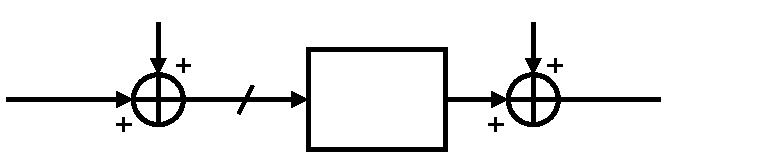
\includegraphics[scale=0.70000]{./figs/dco_noise.pdf}\\
   % translate x=-384 y=320 scale 0.38
   \putbox{1.02900in}{0.39200in}{0.96}{u[n]}%
   \putbox{1.48400in}{0.24500in}{0.96}{$\frac{2\pi K_{DCO}T}{1-z^{-1}}$}%
   \putbox{2.66700in}{0.34300in}{0.96}{$\Phi_{out}$[n]}%
   \putbox{0.78400in}{0.60900in}{0.96}{q$_{OTW}$[n]}%
   \putbox{0.18200in}{0.37800in}{0.96}{$\hat{\textnormal{u}}$[n]}%
   \putbox{2.54800in}{0.62300in}{0.96}{$\Phi_{n_{DCO}}$[n]}%
   } % close 'parbox'
   } % close 'scalebox'
   \vspace{-\baselineskip} % this is not necessary, but looks better
\fontfamily{\rmdefault}\selectfont

	% 	\caption{DCO additive noise model.}
	% 	\label{fig:dco_noise2}
	% \end{figure}
	% \FloatBarrier

	%  Oscillator phase noise due to stochastic and uncorrelated circuit and supply noise can be analyzed as additive voltage disturbance $\delta v_n$ with variance $\sigma_{v_n}^2$ to the oscillator waveform $V_{osc}$ at any given time.  In a stable, noiseless oscillator, amplitude is inherently tied to signal phase, i.e. $V_{osc}(\Phi=\omega t)$. With additive noise, given $\frac{dV_{osc}(\Phi)}{d\Phi}$ is finite $\forall$t, a small voltage disturbance from noise $\delta v_{n}$ will be coupled as a disturbance $\delta\Phi_{n}$ in the oscillator phase, shown in figure \ref{fig:aperture_noise}. The phase evolution of the noisy oscillator for an infinitesimal time increment $\delta t$  with such a disturbance is:
	%  \begin{equation}
	% 	\Phi_{out}(t+\delta t) = \Phi_{out}(t) + \delta\Phi_n + \omega_{osc}\delta t \label{eq:rwalk_ph}
	%  \end{equation}

	% \begin{figure}[htb!]
	% 	\center\fontfamily{\sfdefault}\selectfont
% XCircuit output "aperture_noise.tex" for LaTeX input from aperture_noise.ps
\def\putbox#1#2#3#4{\makebox[0.00000in][l]{\makebox[#1][l]{}\raisebox{\baselineskip}[0.00000in][0.00000in]{\raisebox{#2}[0.00000in][0.00000in]{\scalebox{#3}{#4}}}}}
\def\rightbox#1{\makebox[0.00000in][r]{#1}}
\def\centbox#1{\makebox[0.00000in]{#1}}
\def\topbox#1{\raisebox{-0.60\baselineskip}[0.00000in][0.00000in]{#1}}
\def\midbox#1{\raisebox{-0.20\baselineskip}[0.00000in][0.00000in]{#1}}
   \scalebox{1}{
   \normalsize
   \parbox{4.06875in}{
   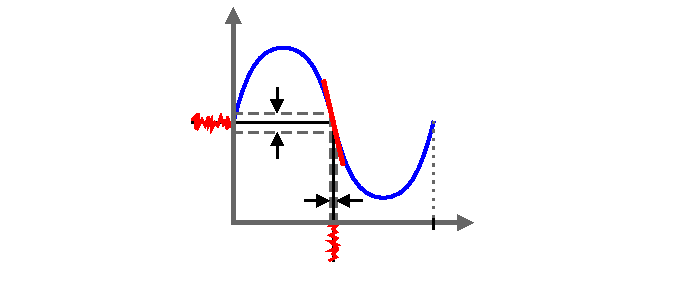
\includegraphics[scale=0.90000]{./figs/aperture_noise.pdf}\\
   % translate x=96 y=256 scale 0.38
   \putbox{2.82600in}{0.23400in}{0.96}{\rotatebox{-360}{$\Phi$}}%
   \putbox{1.19700in}{1.47600in}{0.96}{V}%
   \putbox{1.58400in}{1.21500in}{0.96}{$\sigma_{v_n}$}%
   \putbox{1.56600in}{0.48600in}{0.96}{$\sigma_{\Phi_n}$}%
   \putbox{1.00800in}{1.13400in}{0.60}{Thermal }%
   \putbox{1.08000in}{1.04400in}{0.60}{noise}%
   \putbox{1.66500in}{0.21600in}{0.60}{Phase }%
   \putbox{1.68300in}{0.12600in}{0.60}{noise}%
   \putbox{2.54700in}{0.21600in}{0.60}{\rotatebox{-360}{$2\pi$}}%
   \putbox{1.35900in}{0.21600in}{0.60}{$0$}%
   \putbox{0.90900in}{0.93600in}{0.96}{$\delta_{v_n}$}%
   \putbox{2.06100in}{0.09000in}{0.96}{$\delta_{\Phi_n}$}%
   \putbox{2.03400in}{0.90900in}{0.96}{$\frac{dV_{osc}(\Phi)}{d\Phi}$}%
   \putbox{1.62900in}{1.45800in}{0.60}{\rotatebox{-360}{$V_{osc}$}}%
   } % close 'parbox'
   } % close 'scalebox'
   \vspace{-\baselineskip} % this is not necessary, but looks better
\fontfamily{\rmdefault}\selectfont

	% 	\caption{Voltage to phase noise conversion.}
	% 	\label{fig:aperture_noise}
	% \end{figure}
	% \FloatBarrier
	%   Assuming $\delta v_n$ is Gaussian white noise, $\delta\Phi_{n}$ is sampled stochastically at any instant based on the probability distribution \ref{eq:osc_rw_dist}, dependent on the current oscillator phase $\Phi_{out}$ and the noiseless voltage-phase relation $V_{osc}(\Phi)$. It will be assumed that like the source noise $\delta v_n$, $\delta\Phi_{n}$ is white spectrum.
	%  \begin{equation}
	%  	P(\delta\Phi_{n}|\Phi_{out}) = \text{Norm}\left(\mu=0, \sigma=\sigma_{v_n}\left(\left.\frac{dV_{osc}(\Phi)}{d\Phi}\right\vert_{\Phi=\Phi_{out}}\right)^{-1}\right) \label{eq:osc_rw_dist}
	%  \end{equation} 
	% Spectral analysis of the noisy oscillator phase can be made utilizing discrete time-modeling. Converting \ref{eq:rwalk_ph} into a sampled signal with time step $\delta t$ 
	% \begin{equation}
	% 	\Phi_{out}[n+1] = \Phi_{out}[n] + \omega_{osc}\delta t + \delta\Phi_n[n|\Phi_{out}[n]]
	% \end{equation}
	% Computing the z-transform, and splitting the result into the oscillation $\Phi_{osc}$ and phase noise $\Phi_{n}$ components:
	% \begin{equation}
	% 	\Phi_{out}(z) = \frac{\omega_{osc}\delta t}{z-1} + \frac{\delta\Phi_n(z)}{z-1} = \Phi_{osc}(z) + \Phi_{n}(z)
	% \end{equation}
	% \begin{equation}
	% 	\Rightarrow \Phi_{n}(z) = \frac{\delta\Phi_n(z)}{z-1} \label{eq:z_osc_pn}
	% \end{equation}
	% Application of the bilinear transform to \ref{eq:z_osc_pn} can be used to approximate the continuous phase noise spectrum, if $s=j\omega$
	% \begin{equation}
	% 	\Phi_{n}(s) = \left.\Phi_{n}(z)\right\vert_{z=1-s\delta t} = \left.\frac{\delta\Phi_n(z)}{z-1}\right\vert_{z=1+s\delta t} = \frac{\delta\Phi_n(s)}{s\delta t}
	% \end{equation}
	% The phase noise PSD is therefore:
	% \begin{equation}
	% 	S_{\Phi n_{DCO}}(f)= \lim_{\Delta T\rightarrow\infty}\frac{1}{\Delta T}\left|\frac{\delta\Phi_n(j2\pi f)}{j2\pi f \delta t}*\mathcal{F}\left\{\text{rect}\left(\frac{t}{\Delta t}\right)\right\}\right|^2  =  \frac{S_{0\Phi n_{DCO}}}{f^2}
	% \end{equation}
	% Following that the phase disturbance signal $\delta\Phi_{n}(t)$ is white spectrum, a constant value for its PSD $S_{0\Phi n_{DCO}}$ can be defined. The value for $S_{0\Phi n_{DCO}}$ is highly dependent on implementation and is best extracted by means of curve fitting simulation or physical measurement.
